\documentclass[
	% -- opções da classe memoir --
	12pt,				% tamanho da fonte
	openright,			% capítulos começam em pág ímpar (insere página vazia caso preciso)
	twoside,			% para impressão em recto e verso. Oposto a oneside
	a4paper,			% tamanho do papel. 
	% -- opções da classe abntex2 --
	%chapter=TITLE,		% títulos de capítulos convertidos em letras maiúsculas
	%section=TITLE,		% títulos de seções convertidos em letras maiúsculas
	%subsection=TITLE,	% títulos de subseções convertidos em letras maiúsculas
	%subsubsection=TITLE,% títulos de subsubseções convertidos em letras maiúsculas
	% -- opções do pacote babel --
	english,			% idioma adicional para hifenização
	french,				% idioma adicional para hifenização
	spanish,			% idioma adicional para hifenização
	brazil,				% o último idioma é o principal do documento
	]{abntex2}


% ---
% Pacotes
% ---
\usepackage{lmodern}			% Usa a fonte Latin Modern
\usepackage[T1]{fontenc}		% Seleção de codigos de fonte.
\usepackage[utf8]{inputenc}		% Codificação do documento (conversão automática dos acentos)
\usepackage{indentfirst}		% Indenta o primeiro parágrafo de cada seção.
\usepackage{color}				% Controle das cores
\usepackage{graphicx}			% Inclusão de gráficos
\usepackage{microtype} 			% para melhorias de justificação
\usepackage{float}
\usepackage{mathabx}
\usepackage[ampersand]{easylist}

\usepackage{multicol}
\usepackage{multirow}

\usepackage{lipsum}

\usepackage[brazilian,hyperpageref]{backref}
\usepackage[alf]{abntex2cite}


% --- 
% CONFIGURAÇÕES DE PACOTES
% --- 

% ---
% Configurações do pacote backref
% Usado sem a opção hyperpageref de backref
\renewcommand{\backrefpagesname}{Citado na(s) página(s):~}
% Texto padrão antes do número das páginas
\renewcommand{\backref}{}

% ---
% Informações de dados para CAPA e FOLHA DE ROSTO
% ---
\titulo{Implementação de uma Unidade Lógica Aritmética com Portas Lógicas Básicas}
\autor{Atílio Antônio Dadalto \\ Vitor Ferraz Matos Brunoro}
\local{Vitória}
\data{2018}
\instituicao{%
  Universidade Federal do Espírito Santo
  \par Departamento de Informática}
\tipotrabalho{Relatório}
\preambulo{Relatório apresentado como requisito parcial para obtenção de nota na disciplina de Elementos de Lógica Digital, pela Universidade Federal do Espírito Santo.}

\usepackage[LGRgreek]{mathastext}

% alterando o aspecto da cor azul
\definecolor{blue}{RGB}{41,5,195}

% informações do PDF
\makeatletter
\hypersetup{
     	%pagebackref=true,
		pdftitle={\@title}, 
		pdfauthor={\@author},
    	pdfsubject={\imprimirpreambulo},
	    pdfcreator={LaTeX with abnTeX2},
		pdfkeywords={abnt}{latex}{abntex}{abntex2}{relatório técnico}, 
		colorlinks=true,       		% false: boxed links; true: colored links
    	linkcolor=blue,          	% color of internal links
    	citecolor=blue,        		% color of links to bibliography
    	filecolor=magenta,      		% color of file links
		urlcolor=blue,
		bookmarksdepth=4
}
\makeatother

% O tamanho do parágrafo é dado por:
\setlength{\parindent}{1.3cm}

% Controle do espaçamento entre um parágrafo e outro:
\setlength{\parskip}{0.2cm}  % tente também \onelineskip

% ----
% Início do documento
% ----
\begin{document}

% Seleciona o idioma do documento (conforme pacotes do babel)
%\selectlanguage{english}
\selectlanguage{brazil}

% Retira espaço extra obsoleto entre as frases.
\frenchspacing 

% ---
% Capa
% ---
\imprimircapa

\imprimirfolhaderosto

\tableofcontents*

% ----------------------------------------------------------
% ELEMENTOS TEXTUAIS
% ----------------------------------------------------------
\textual

% ----------------------------------------------------------
% COMEÇO DO TEXTO
% ----------------------------------------------------------
\chapter*[Introdução]{Introdução}
\addcontentsline{toc}{chapter}{Introdução}

Neste projeto, buscamos implementar todas as funções necessárias para a composição de uma Unidade Lógica e Aritmética que opere em 16 bits, além de uma calculadora com seu próprio display hexadecimal de saída, tomando como ferramenta o software utilizado durante o curso, \textit{Logisim}.

Através da modularidade, foi possível utilizar a abordagem de dividir para conquistar, tornando o projeto como um todo mais organizado e manutenível. Isso provou-se notadamente útil na construção do multiplexador 8:1 com entrada de 8 bits (\autoref{mux818}), por exemplo.

Este relatório documenta a trajetória da construção dessa Unidade Lógica e Aritmética através de portas lógicas básicas, de duas entradas, pontuando as sub-funções elaboradas e como foram integradas, bem como os testes efetuados, estes no \autoref{apendiceA}.


\chapter{Operações}\label{operacoes}

\section{ADD bit a bit \texorpdfstring{$A+B$}{Lg}}

Primeiramente, antes de implementar o somador de duas entradas de 8 bits, estabelecemos um somador completo, para que seja possível o transporte de entrada que um meio somador não é suficiente para realizar. Desse modo, agora temos A, B e o \textit{carry-in}, que resultarão nas saídas S (soma dos algarismos) e \textit{carry-out} (transporte de saída). O \textit{full adder} está representado na \autoref{somador1b}:

\begin{figure}[H]
	\begin{center}
	    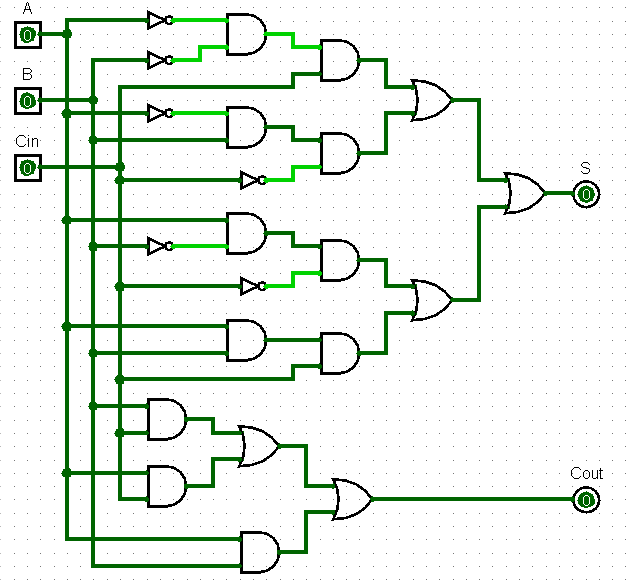
\includegraphics[scale=0.5]{somador1b.png}
	\end{center}
\caption{\label{somador1b}Circuito do somador completo de 1 bit}
\end{figure}

A partir desse circuito, podemos utilizá-lo como caixa preta e, com isso, criar um somador para entradas de 8 bits. Assim, temos:

\begin{figure}[H]
	\begin{center}
	    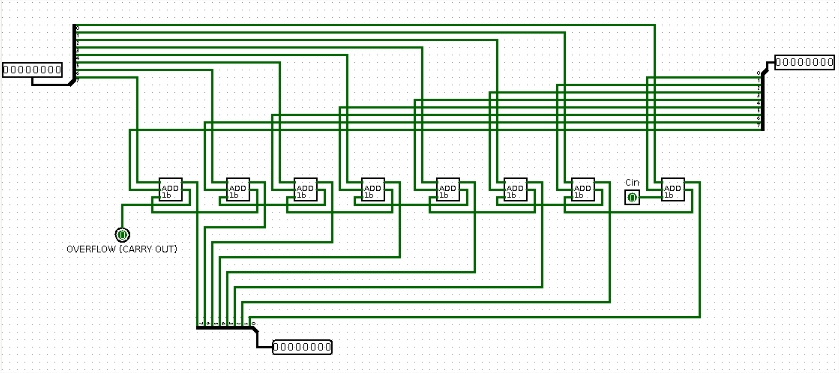
\includegraphics[scale=0.5]{somador8b.jpg}
	\end{center}
\caption{\label{somador8b}Circuito do somador completo de 8 bits}
\end{figure}

\section{SUB bit a bit \texorpdfstring{$A-B$}{Lg}}
Para realizar a subtração com duas entradas de 8 bits, usaremos a mesma lógica exercitada na implementação do somador acima. Em primeiro lugar, é preciso construir um subtrator completo que seja capaz de processar a entrada do transporte em hipóteses de “empresta” 1. Portanto, temos novamente como entradas A, B e o transporte de entrada. Já na saída, o resultado da subtração e o transporte de saída. O subtrator completo está representado na \autoref{subtrator1b}:

\begin{figure}[H]
	\begin{center}
	    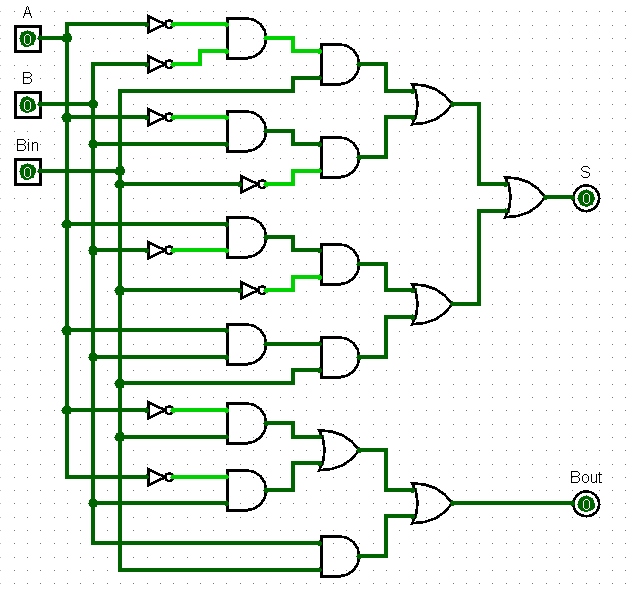
\includegraphics[scale=0.4]{subtrator1b.png}
	\end{center}
\caption{\label{subtrator1b}Circuito do subtrator completo de 1 bit}
\end{figure}

Utilizaremos o circuito acima como caixa preta e, por consequência, poderemos implementar um subtrator agora para entradas de 8 bits:

\begin{figure}[H]
	\begin{center}
	    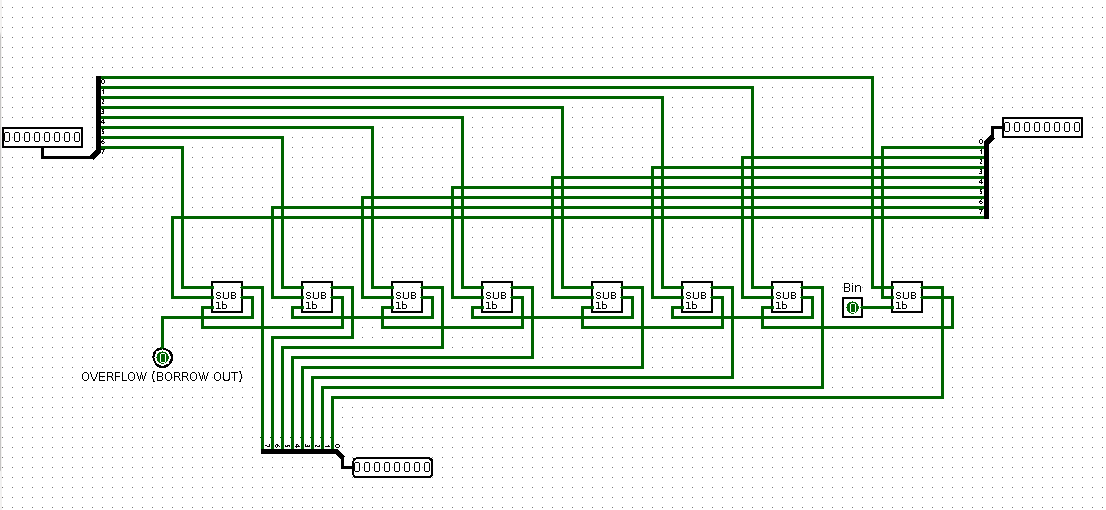
\includegraphics[scale=0.4]{subcircuito.png}
	\end{center}
\caption{\label{subtrator8b}Circuito do subtrator completo de 8 bits}
\end{figure}

\section{XOR bit a bit \texorpdfstring{$A \oplus B$}{Lg}}
Na operação XOR (‘ou exclusivo’) bit a bit, temos a possibilidade de 0 ou 1 como valor de cada bit, sendo que se aplicarmos essa operação em bits de mesmo valor, a saída é 0. Se diferentes, a saída é 1. Para entradas de 8 bits, implementamos o circuito abaixo:

\begin{figure}[H]
	\begin{center}
	    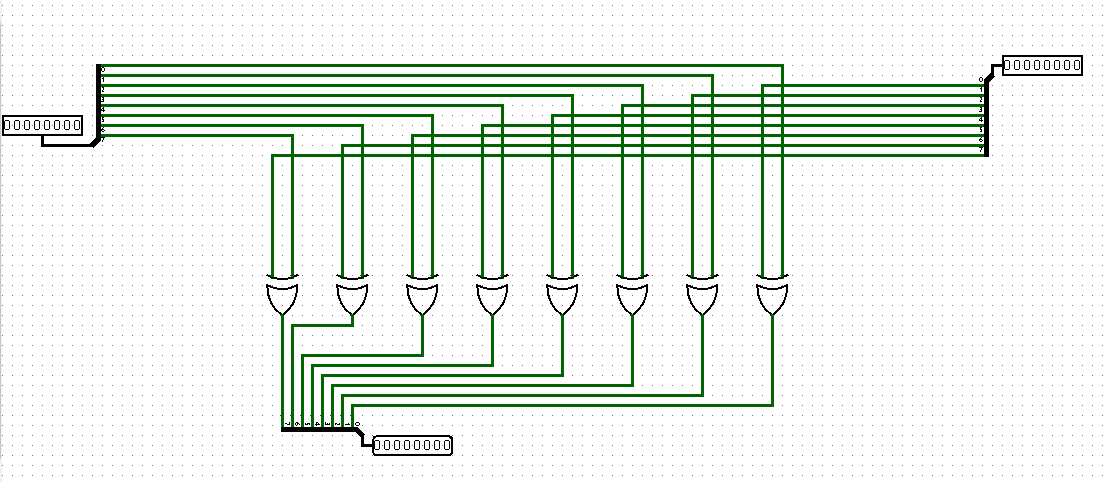
\includegraphics[scale=0.4]{xorcircuito.png}
	\end{center}
\caption{\label{xor}Circuito do ‘ou exclusivo’ de 8 bits}
\end{figure}

\section{OR bit a bit \texorpdfstring{$A+B$}{Lg}}

Na operação OR (‘ou’) bit a bit, temos a possibilidade de 0 ou 1 como valor de cada bit, bastando um bit ter o valor 1 para que a saída também seja 1. Se ambos os bits tiverem valor 0, a saída é 0. Para operações com entradas de 8 bits, temos o seguinte circuito:

\begin{figure}[H]
	\begin{center}
	    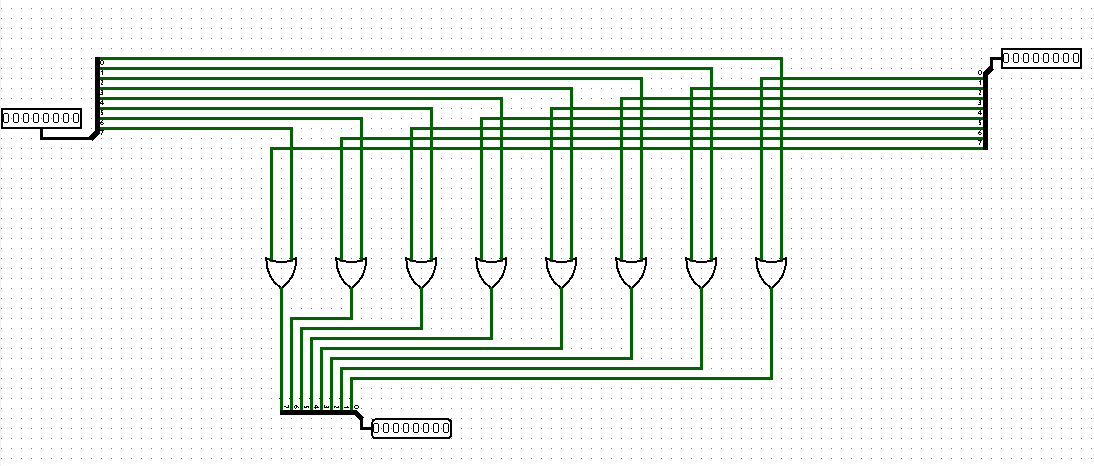
\includegraphics[scale=0.4]{orcircuito.png}
	\end{center}
\caption{\label{or}Circuito do ‘OR bit a bit’ de 8 bits.}
\end{figure}

\section{AND bit a bit \texorpdfstring{$A\cdot B$}{Lg}}

Na operação AND (‘e’) bit a bit, temos a possibilidade de 0 ou 1 como valor de cada bit, sendo necessário que os dois bits sejam 1 para que a saída também seja 1. Em qualquer outra hipótese, a saída é 0. Posto isso, vejamos o circuito para essa operação em 8 bits:

\begin{figure}[H]
	\begin{center}
	    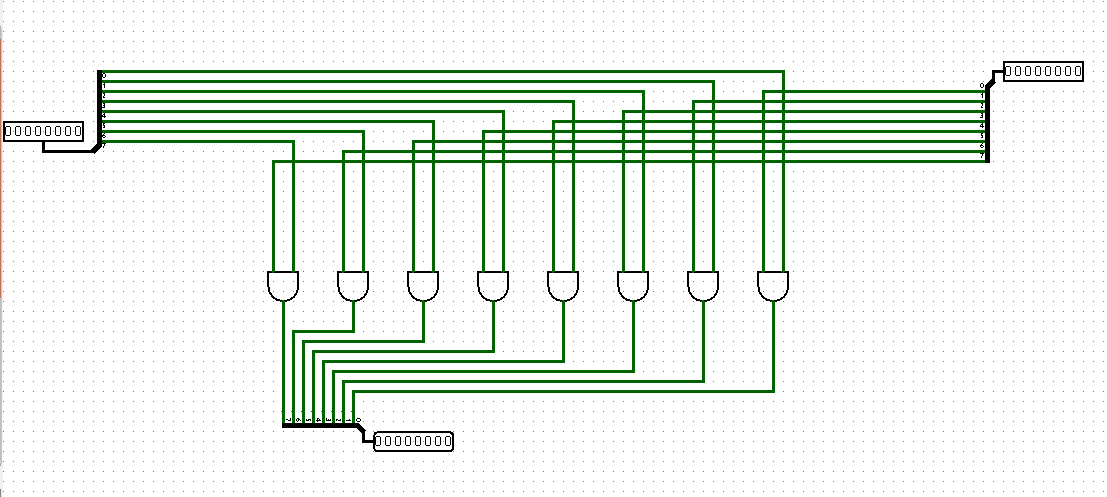
\includegraphics[scale=0.4]{andcircuito.png}
	\end{center}
\caption{\label{and}Circuito do ‘AND bit a bit’ de 8 bits.}
\end{figure}

\section{SHL \texorpdfstring{$A << 1$}{Lg}}

O shift left é uma instrução que desloca todos os bits de A para a esquerda, multiplicando o número por 2. O circuito dessa instrução de deslocamento pode ser implementado desta maneira:

\begin{figure}[H]
	\begin{center}
	    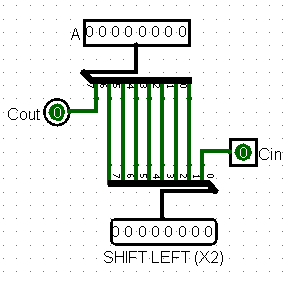
\includegraphics[scale=0.6]{shiftleft.png}
	\end{center}
\caption{\label{shl}Circuito do 'shift left'}
\end{figure}


\section{SHR \texorpdfstring{$A >> 1$}{Lg}}

O shift right, por sua vez, é uma instrução que desloca todos os bits de A para a direita, dividindo o número por 2. Vejamos:

\begin{figure}[H]
	\begin{center}
	    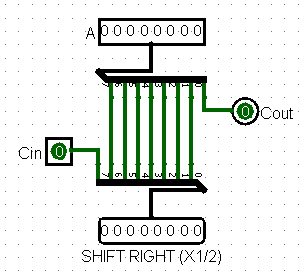
\includegraphics[scale=0.6]{shiftright.png}
	\end{center}
\caption{\label{shr}Circuito do 'shift right'}
\end{figure}



\chapter{A Unidade Lógica e Aritmética}

Ao empregar conceitos de modularização, podemos agora projetar uma Unidade Lógica Aritmética (ULA) que compute o resultado de todas as operações acima elencadas. Para isso, é imperiosa a implementação de um multiplexador que realizará a função primordial de selecionar qual das operações a ser realizada com os operandos de 8 bits. 

\section{Multiplexadores}

Antes de chegar no multiplexador que seleciona a operação a ser realizada pela ULA, começamos com um multiplexador básico 2:1, e, a partir dele, utilizamos a modularidade de circuitos até chegarmos no multiplexador 8:1 para operandos de 8 bits. Os circuitos são sucessivamente utilizados como caixa preta. Isto posto, temos os seguintes multiplexadores:

\begin{figure}[H]
	\begin{center}
	    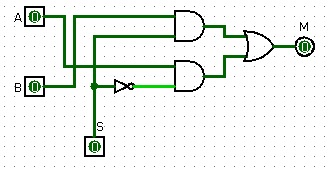
\includegraphics[scale=0.6]{mux21.png}
	\end{center}
\caption{\label{mux21}Circuito do multiplexador 2:1 para operandos de 1 bit}
\end{figure}

\begin{figure}[H]
	\begin{center}
	    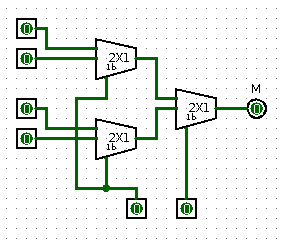
\includegraphics[scale=0.6]{mux41.png}
	\end{center}
\caption{\label{mux41}Circuito do multiplexador 4:1 para operandos de 1 bit}
\end{figure}

\begin{figure}[H]
	\begin{center}
	    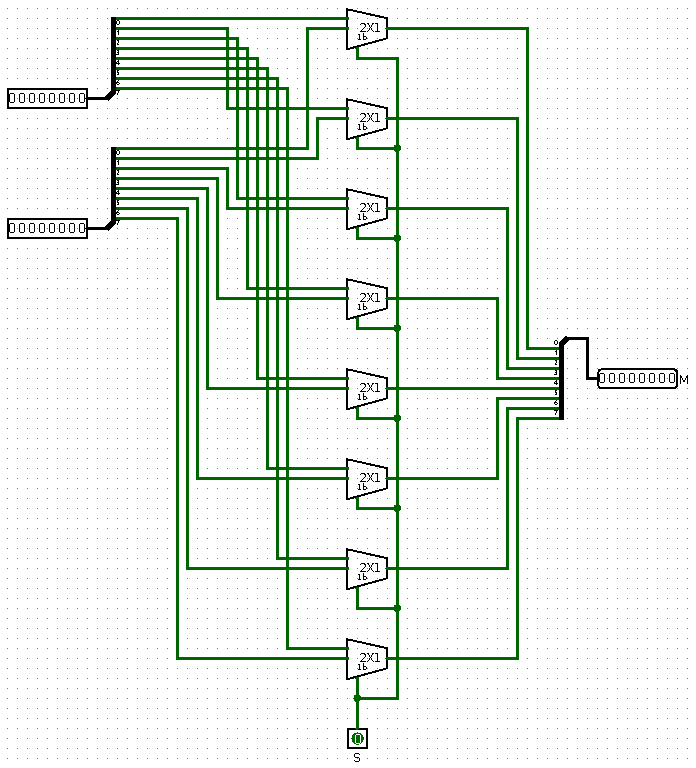
\includegraphics[scale=0.5]{mux218.png}
	\end{center}
\caption{\label{mux218}Circuito do multiplexador 2:1 para operandos de 8 bits}
\end{figure}

\begin{figure}[H]
	\begin{center}
	    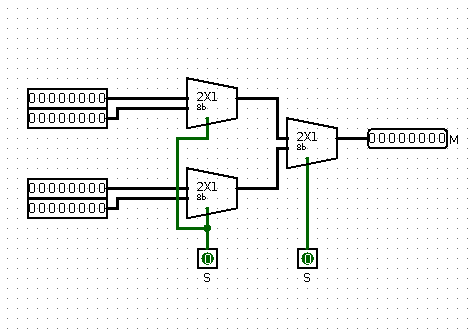
\includegraphics[scale=0.6]{mux418.png}
	\end{center}
\caption{\label{mux418}Circuito do multiplexador 4:1 para operandos de 8 bits}
\end{figure}

\begin{figure}[H]
	\begin{center}
	    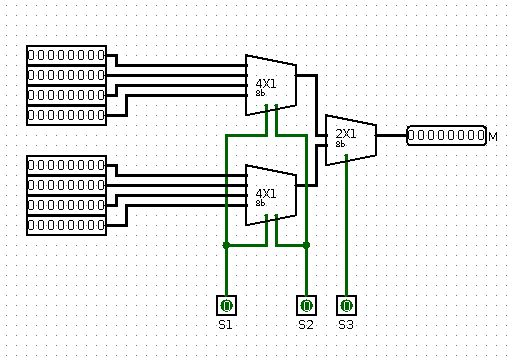
\includegraphics[scale=0.7]{mux818.png}
	\end{center}
\caption{\label{mux818}Circuito do multiplexador 8:1 para operandos de 8 bits}
\end{figure}

Os multiplexadores possuem papel fundamental na elaboração deste projeto, uma vez que nos permitem escolher dentre várias opções de saída. Não apenas utilizados para a seleção da saída S, também foram aplicados para selecionar a saída C, uma vez que existem 4 diferentes opções para o carry-out, a saber, adição, subtração, shift left e shift right.

Com este último multiplexador de 8 bits da \autoref{mux818}, é possível selecionar a saída desejada dentre as sete saídas das operações descritas no \autoref{operacoes}. A 8ª opção, por não ser utilizada pela ULA, foi aterrada.

\section{A saída Z (zero)}

Para gerar a saída Z, ligamos a saída S em um novo circuito ZERO, que pode ser descrito como uma grande porta NOR com entrada de 8 bits. Ele é visto na \autoref{saidaZ}.

\begin{figure}[H]
	\begin{center}
	    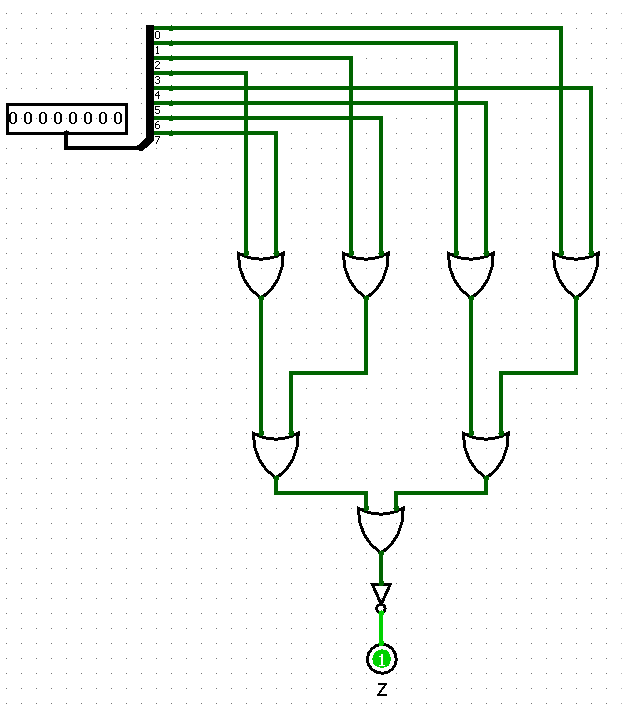
\includegraphics[scale=0.5]{ZERO.png}
	\end{center}
\caption{\label{saidaZ}Circuito que calcula se todos os bits da saída S são 0}
\end{figure}

\section{A saída C (\textit{carry-out})}

Para a saída de \textit{carry-out}, utilizamos um multiplexador 4:1 de 1 bit com o \textit{switch} definido pela entrada OP. Dessa forma, ele é capaz de selecionar o \textit{carry-out} dentre as quatro operações. Ao juntar sua saída com a saída do próximo circuito apresentado em uma porta AND, teremos a saída C desejada.

\subsection{VALIDA\_COUT}

No entanto, ao efetuar os cálculos, é notável, sobretudo quando operações sem \textit{carry-out} eram escolhidas, a ocorrência de saída de \textit{carry-out} de operações que não foram selecionadas, como pode ser observado no recorte da \autoref{carryoutincorreto}. Para corrigir isso, foi implementado o circuito VALIDA\_COUT, visto na \autoref{validacout}.


\begin{figure}[H]
	\begin{center}
	    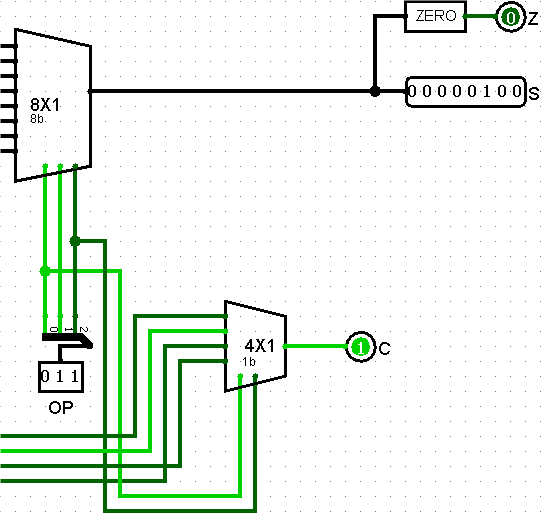
\includegraphics[scale=0.5]{carryoutincorreto.png}
	\end{center}
\caption{\label{carryoutincorreto}Por reutilizarmos a entrada OP para determinar o carry-out, uma saída incorreta foi gerada. Note que a operação escolhida (OR) \textit{não} possui carry-out sob hipótese alguma}
\end{figure}

\begin{figure}[H]
	\begin{center}
	    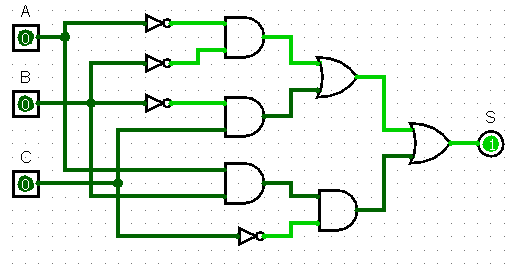
\includegraphics[scale=0.5]{validacout.png}
	\end{center}
\caption{\label{validacout}Circuito que impede \textit{carry-out} inadequado.}
\end{figure}

\begin{figure}[H]
	\begin{center}
	    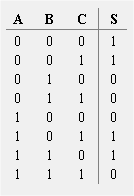
\includegraphics[scale=0.8]{validacouttab.png}
	\end{center}
\caption{\label{validacouttab}Tabela verdade do VALIDA\_COUT.}
\end{figure}

Como podemos ver na tabela da \autoref{validacouttab}, utilizada para a confecção do circuito, a saída é 1 apenas se alguma operação com \textit{carry-out} é selecionada, i.e. soma, subtração, shift left ou shift right. Com isso e o multiplexador, agora possuímos uma saída C coerente.

\section{A saída S (resultado da operação)}
Finalmente, a saída S é resultado da conexão entre as saídas de todas as operações citadas na \autoref{operacoes} e um multiplexador de 8:1 de 8 bits visto na \autoref{mux818}. O resultado a ser exibido estará de acordo com a entrada OP de 3 bits, que serve como \textit{switch} para o multiplexador. 

\section{O circuito da Unidade Lógica Aritmética de 8 bits}

Ao combinar todos os circuitos das operações vistas na \autoref{operacoes} junto com um multiplex 8:1 para operandos de 8 bits, construímos a nossa ULA, tendo esta as supracitadas saídas S, C e Z. O circuito dessa ULA está representado abaixo:

\begin{figure}[H]
	\begin{center}
	    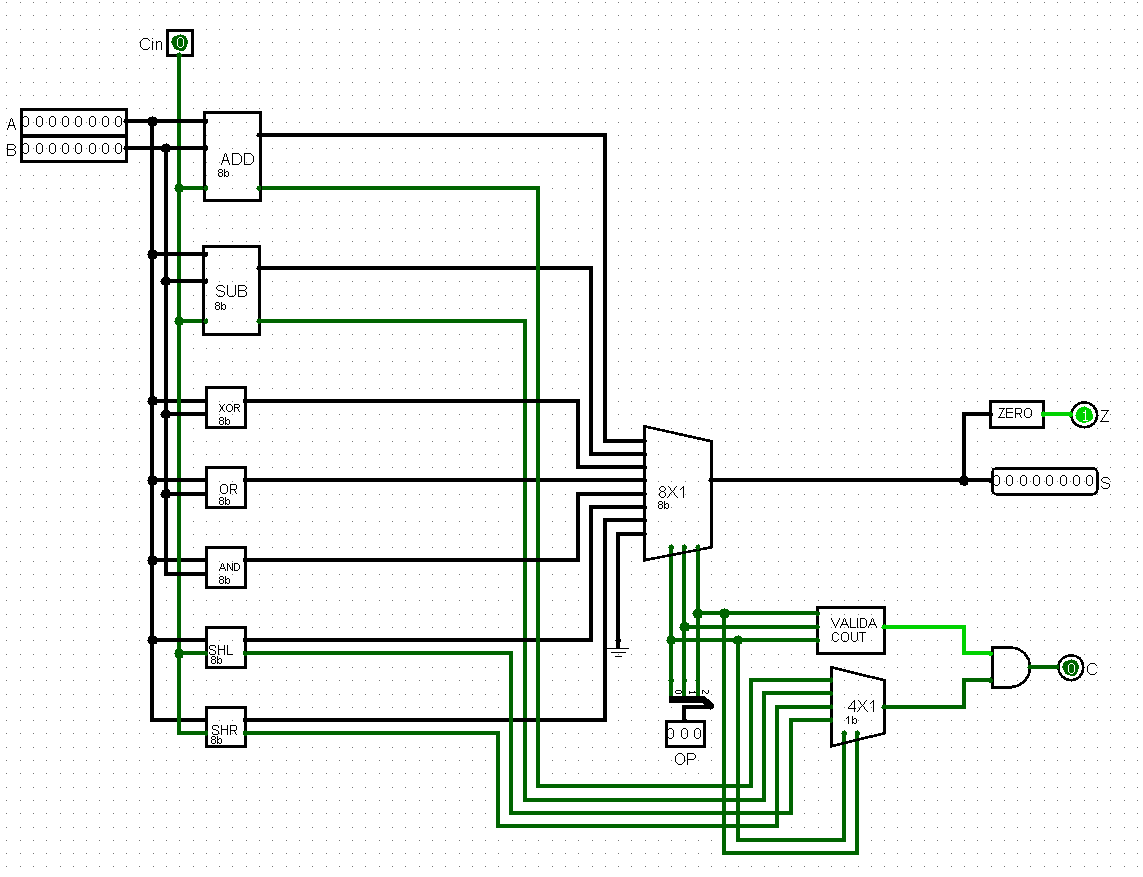
\includegraphics[scale=0.4]{alu8.png}
	\end{center}
\caption{\label{ula8}Circuito da ULA de 8 bits.}
\end{figure}



\chapter{Calculadora}

Agora que construímos uma ULA, podemos colocá-la em caixa preta, e, assim, utilizá-la para criar novos circuitos combinacionais. Posto isso, usaremos essa ULA junta de dois decodificadores idênticos para elaborar uma calculadora, cuja saída será representada em dois dígitos hexadecimais em displays de 7 segmentos. Mantivemos a saída x (ponto) no circuito do decodificador, mesmo que este segmento esteja sempre desligado, como pode ser visto na \autoref{decodetabela}.

\section{Decodificador}
Para a criação do decodificador, relacionamos uma entrada de 4 bits (para todos os dígitos hexadecimais) com todos os segmentos do display. Através da ferramenta de análise combinacional do software \textit{Logisim}, foi possível facilmente implementar o decodificador através de portas de duas entradas apenas. 

\begin{figure}[H]
	\begin{center}
	    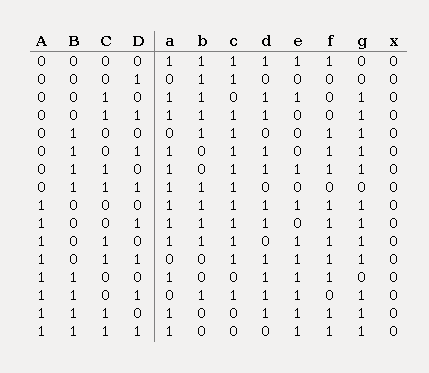
\includegraphics[scale=0.8]{decodetab.png}
	\end{center}
\caption{\label{decodetabela}Tabela verdade do decodificador.}
\end{figure}


\begin{figure}[H]
	\begin{center}
	    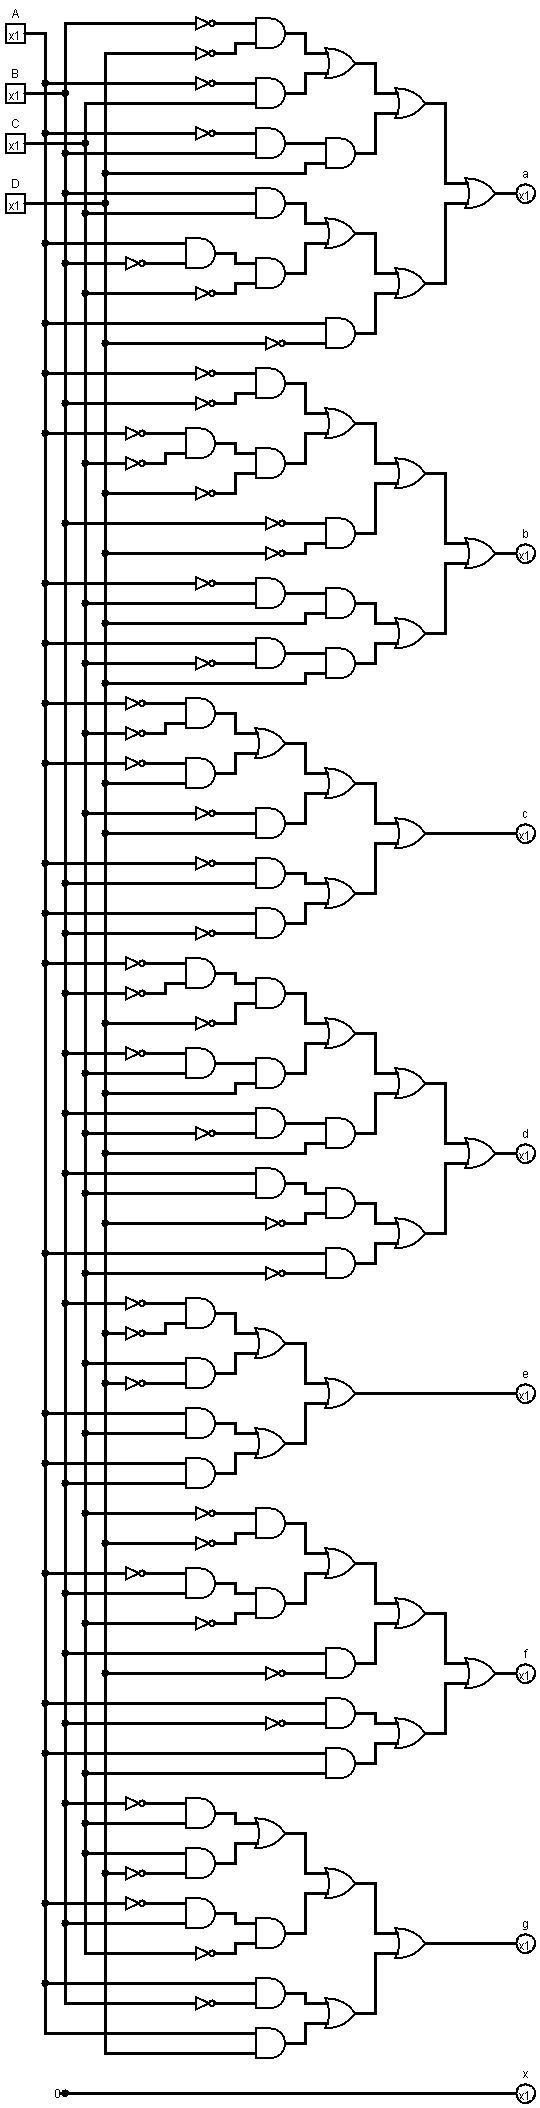
\includegraphics[scale=0.3]{decode.png}
	\end{center}
\caption{\label{decode}Circuito do decodificador.}
\end{figure}

\section{Circuito da calculadora}
\begin{figure}[H]
	\begin{center}
	    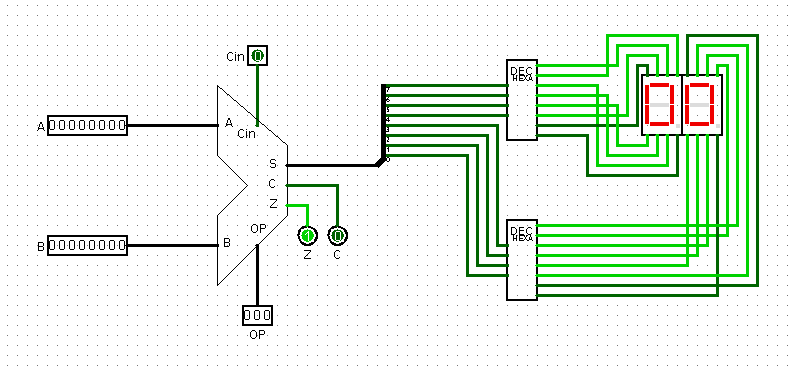
\includegraphics[scale=0.57]{calc.png}
	\end{center}
\caption{\label{calc}Circuito da calculadora.}
\end{figure}

Como visto na \autoref{calc}, a saída S da ULA é dividida e utilizada pelos decodificadores, que por sua vez estão conectados aos displays de 7 segmentos. Assim, desfrutamos de uma ULA que exibe sua saída em um display hexadecimal.


\chapter{A ULA (16 bits)}

Com a ULA de 8 bits pronta, é possível utilizá-la como caixas pretas e concatená-las a fim de montar uma ULA de 16 bits. Algum cuidado foi necessário com as saídas e entradas, nomeadamente a saída zero, a saída \textit{carry-out} e, consequentemente, a entrada \textit{carry-in}, que, no caso da ULA superior (que opera o byte menos significativo) vista na \autoref{ula16}, depende da saída \textit{carry-out} da ULA inferior (que opera o byte mais significativo).

Em favor da legibilidade do circuito, optamos por não simplificar excessivamente os componentes da ULA de 16 bits, que do contrário tornava-se demasiadamente obscura. No entanto, introduzimos um novo circuito: o CARRY\_SHR, visto na \autoref{opcarry}.

\begin{figure}[H]
	\begin{center}
	    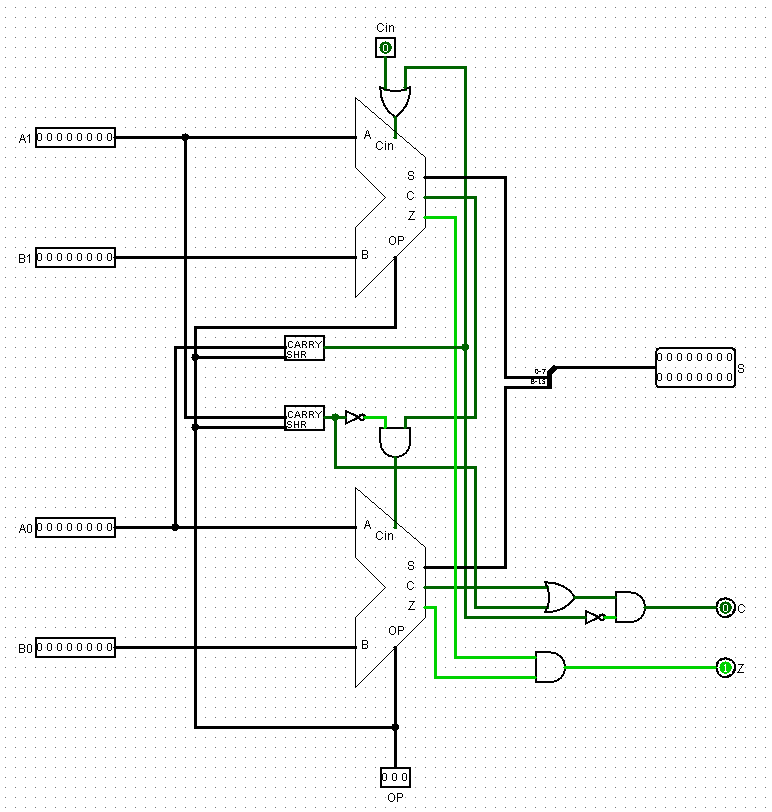
\includegraphics[scale=0.48]{ULA16.png}
	\end{center}
\caption{\label{ula16}Versão final do circuito da ULA de 16 bits.}
\end{figure}
    
\section{Operações com \textit{carry-out}}\label{opcarry}
Como supradito, após concatenar as duas ULAs de 8 bits, fez-se necessário lidar com as saídas de \textit{carry-out} a fim de que o as operações funcionassem da forma correta. A operação de shift right, em especial, precisou ser tratada de acordo para que o cálculo fosse realizado corretamente. 
Para isso, implementamos o seguinte circuito:

\begin{itemize}
  \item  CARRY\_SHR
\end{itemize}

\begin{figure}[H]
	\begin{center}
	    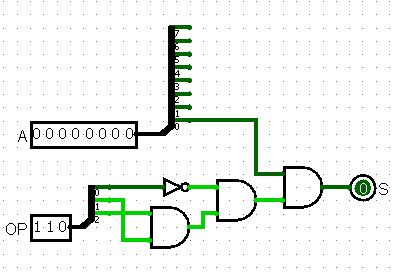
\includegraphics[scale=0.6]{CARRY_SHR.png}
	\end{center}
\caption{\label{carry_shr}Circuito que retorna 1 quando o bit menos  significativo é 1 e a operação de shift right foi escolhida.}
\end{figure}

Este circuito trata os casos em que a operação é de shift right e o bit menos significativo da entrada A é 1. Assim, junto com outras portas lógicas básicas, ele impede que haja carry para o byte mais significativo apenas quando ocorre \textit{carry-out} da operação de shift right (isto é, evita um carry incoerente). Da mesma forma, também utilizamos este circuito para levar o carry do byte mais significativo para o byte menos significativo. 

Além disso, esse mesmo circuito foi capaz de controlar o \textit{carry-out} final, que também apresentava problemas, pois, mesmo havendo transporte interno (para outra ULA), a saída C (transporte final) tornava-se 1. Neste quesito, seu funcionamento é análogo ao do circuito VALIDA\_COUT, visto na \autoref{validacout}, que serve como um ``portão'' para o \textit{carry-out} da ULA de 8 bits, evitando que a saída C torne-se 1 inapropriadamente. Para o controle do carry, utilizamos portas NOT com portas AND, de forma a não alterar o funcionamento da ULA quando o circuito auxiliar retorna 0, como visto na \autoref{ula16}.

Posto isto, possuímos \textit{carry-in} e \textit{carry-out} completamente funcionais, bastando apenas explicar a saída Z e a saída S.

\section{As saídas Z e S}

A saída Z de ambas as ULAs foi intuitivamente unida em uma porta AND, de forma a retornar 1 apenas quando \textit{ambas} as ULAs retornam 1 (saída S igual a zero). No caso das saídas S, estas foram ligadas em uma única saída S de 16 bits.


\chapter*[Conclusão]{Conclusão}
\addcontentsline{toc}{chapter}{Conclusão}

Pelo estudo realizado neste trabalho, fica evidente como podemos chegar a sistemas progressivamente mais complexos, como uma Unidade Lógica e Aritmética, tendo como ponto de partida portas lógicas básicas. Iniciamos o projeto com portas lógicas AND, OR e NOT, de duas entradas, para criar os circuitos aritméticos como o somador completo e o subtrator completo, e, a partir dessas estruturas, utilizamos a modularização e o reuso desses circuitos como caixas pretas para conseguir operar números binários de mais algarismos. Em seguida, também com as portas lógicas básicas, podemos criar as operações lógicas AND, OR e XOR bit a bit, além das instruções de SHIFT LEFT e SHIFT RIGHT.

Posteriormente, apenas com o uso de multiplexadores igualmente construídos com portas lógicas básicas, foi possível integrar todas as operações supracitadas, estruturando, portanto, uma Unidade Lógica e Aritmética de 8 bits. Com esta e o uso de decodificadores, foi possível a implementação de uma calculadora com saída que representa dois dígitos hexadecimais em displays de 7 segmentos. Por outro enfoque, mas lançando mão dos mesmos conceitos, foi possível utilizar a ULA de 8 bits para implementar uma ULA de 16 bits.

\begin{apendicesenv}

\chapter{Testes dos circuitos}\label{apendiceA}

Este apêndice serve como repositório para os testes dos circuitos principais utilizados no projeto.

\section{Operações básicas}
\begin{itemize}

\item {ADD}

\begin{figure}[H]
	\begin{center}
	    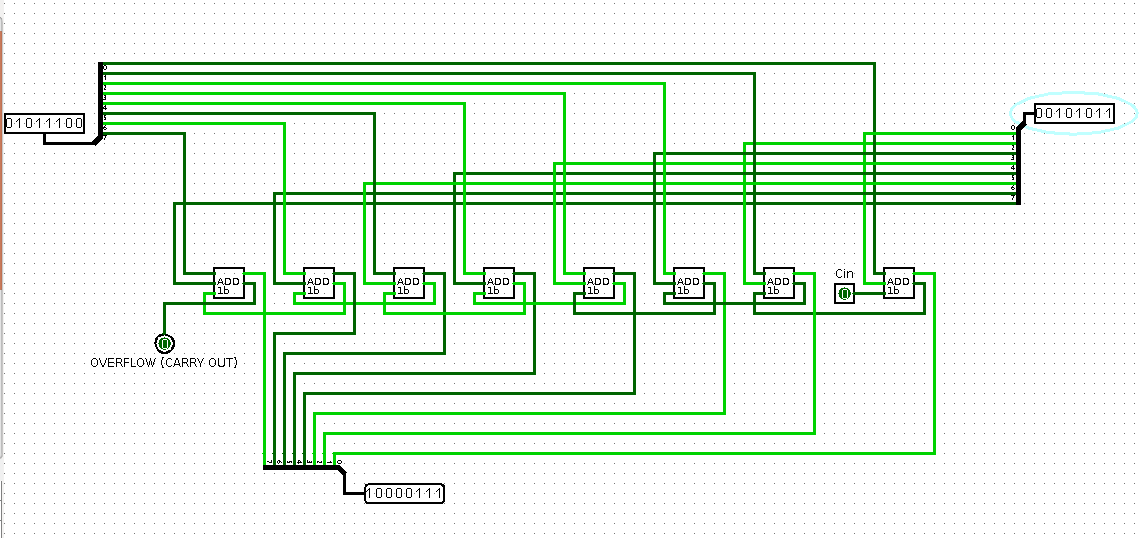
\includegraphics[scale=0.38]{addteste.png}
	\end{center}
\caption{\label{addteste}Exemplo de operação no circuito ADD de 8 bits.}
\end{figure}

\item {SUB}

\begin{figure}[H]
	\begin{center}
	    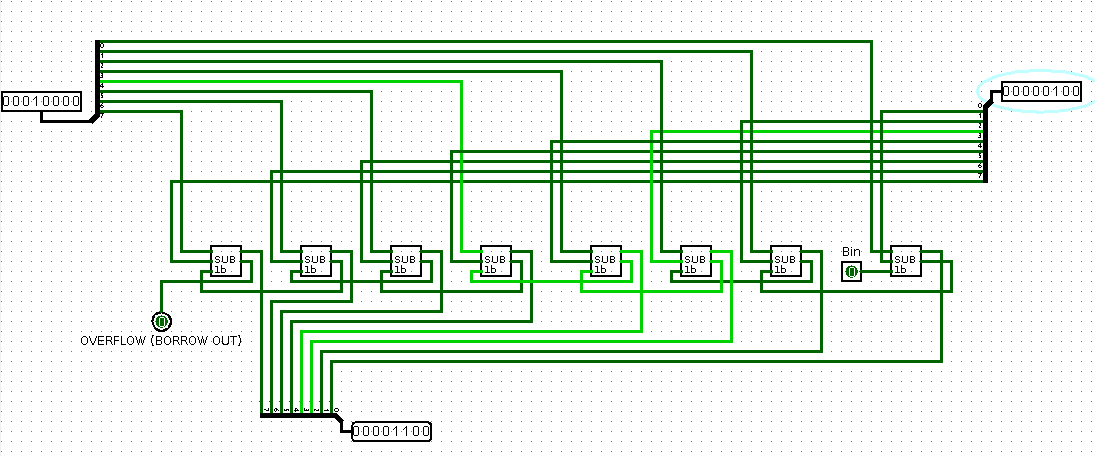
\includegraphics[scale=0.4]{subtratorcompleto.png}
	\end{center}
\caption{\label{subteste}Exemplo de operação no circuito SUB de 8 bits.}
\end{figure}

\item {XOR}

\begin{figure}[H]
	\begin{center}
	    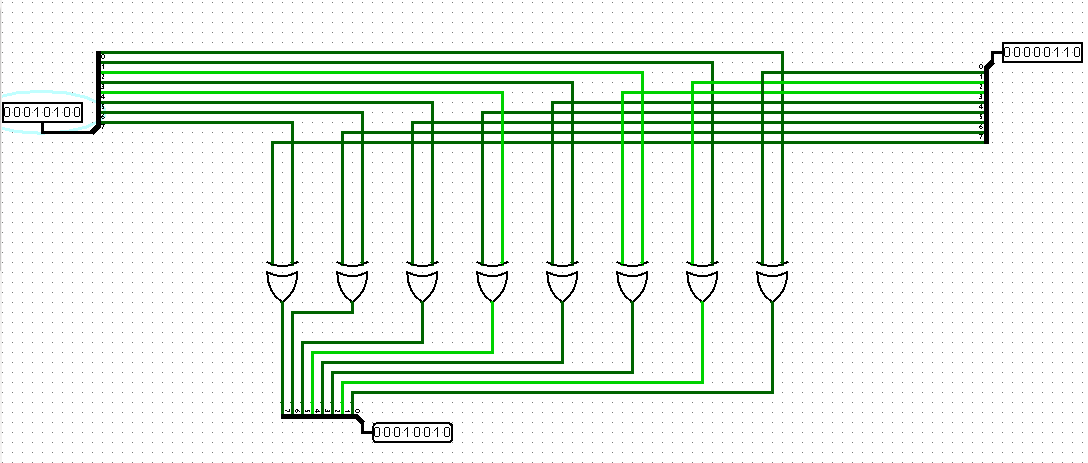
\includegraphics[scale=0.4]{xor8.png}
	\end{center}
\caption{\label{xorteste}Exemplo de operação no circuito XOR de 8 bits.}
\end{figure}

\item {OR}

\begin{figure}[H]
	\begin{center}
	    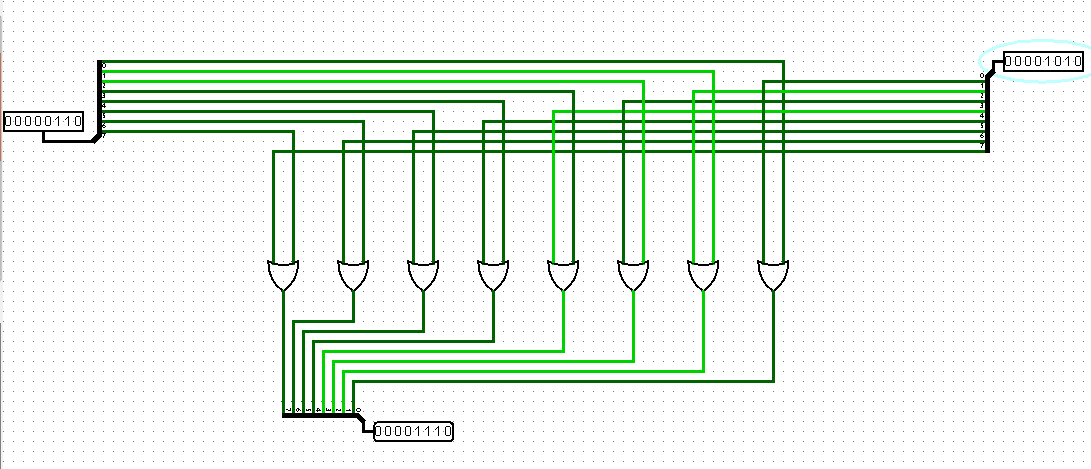
\includegraphics[scale=0.4]{or8.png}
	\end{center}
\caption{\label{orteste}Exemplo de operação no circuito OR de 8 bits.}
\end{figure}

\item {AND}

\begin{figure}[H]
	\begin{center}
	    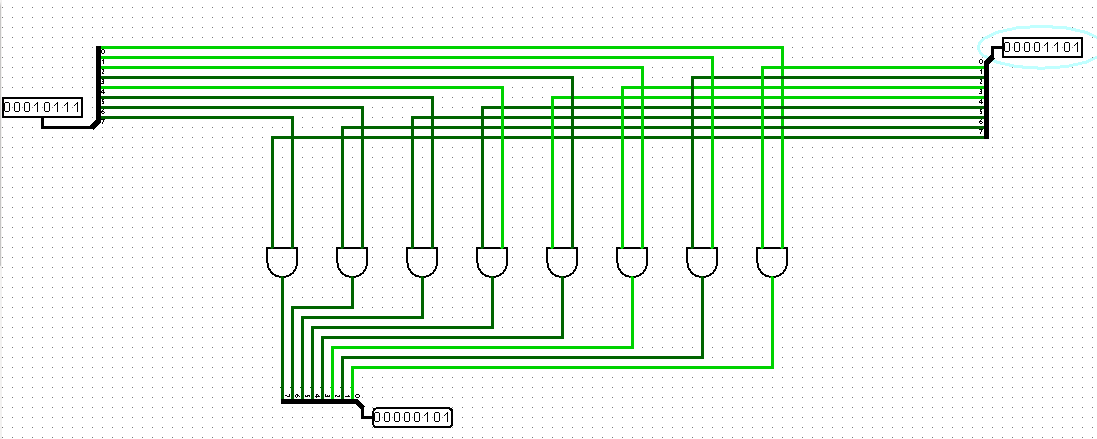
\includegraphics[scale=0.4]{and8.png}
	\end{center}
\caption{\label{andteste}Exemplo de operação no circuito AND de 8 bits.}
\end{figure}

\item {SHL}

\begin{figure}[H]
	\begin{center}
	    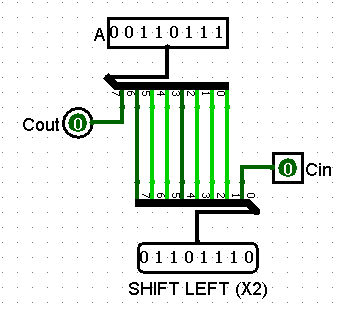
\includegraphics[scale=0.6]{SHLteste.png}
	\end{center}
\caption{\label{shlteste}Exemplo de operação no circuito SHL de 8 bits.}
\end{figure}

\item {SHR}

\begin{figure}[H]
	\begin{center}
	    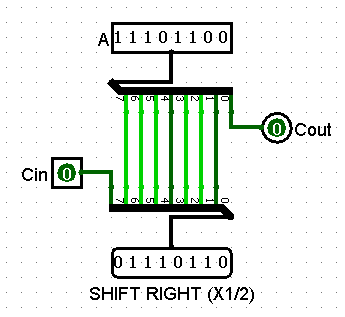
\includegraphics[scale=0.6]{SHRteste.png}
	\end{center}
\caption{\label{shrteste}Exemplo de operação no circuito SHR de 8 bits.}
\end{figure}

\end{itemize}

\newpage
\section{Multiplexadores}

\begin{itemize}
\item {MUX 2:1 1 bit}
\begin{figure}[H]
	\begin{center}
	    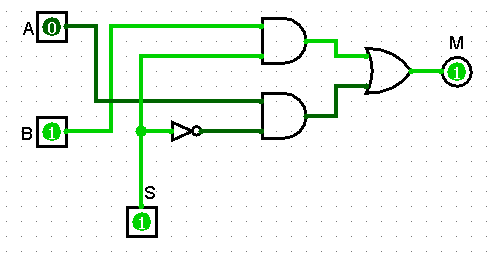
\includegraphics[scale=0.6]{mux211teste.png}
	\end{center}
\caption{\label{mux211teste}Exemplo de escolha no multiplexador 2:1 de 1 bit.}
\end{figure}

\item {MUX 4:1 1 bit}
\begin{figure}[H]
	\begin{center}
	    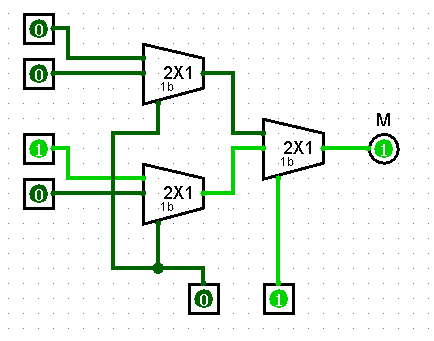
\includegraphics[scale=0.6]{mux411teste.png}
	\end{center}
\caption{\label{mux411teste}Exemplo de escolha no multiplexador 4:1 de 1 bit.}
\end{figure}

\newpage
\item {MUX 8:1 1 bit}
\begin{figure}[H]
	\begin{center}
	    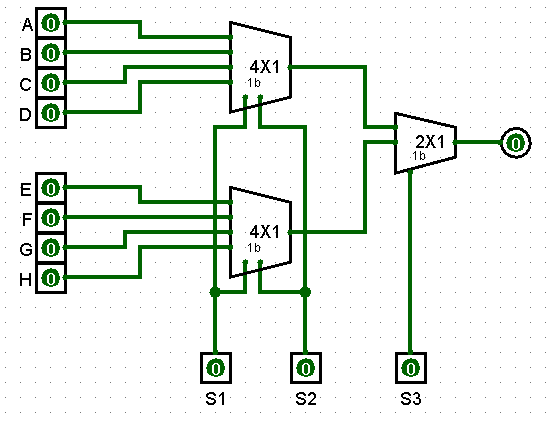
\includegraphics[scale=0.4]{mux811teste.png}
	\end{center}
\caption{\label{mux811teste}Exemplo de escolha no multiplexador 8:1 de 1 bit.}
\end{figure}

\item {MUX 2:1 8 bit}
\begin{figure}[H]
	\begin{center}
	    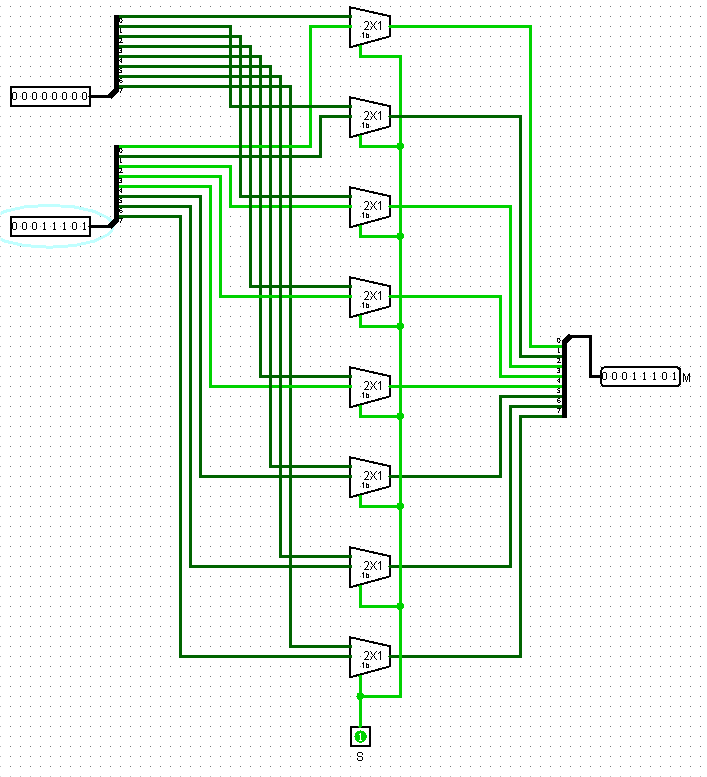
\includegraphics[scale=0.45]{mux218teste.png}
	\end{center}
\caption{\label{mux218teste}Exemplo de escolha no multiplexador 2:1 de 8 bits.}
\end{figure}

\newpage
\item {MUX 4:1 8 bit}
\begin{figure}[H]
	\begin{center}
	    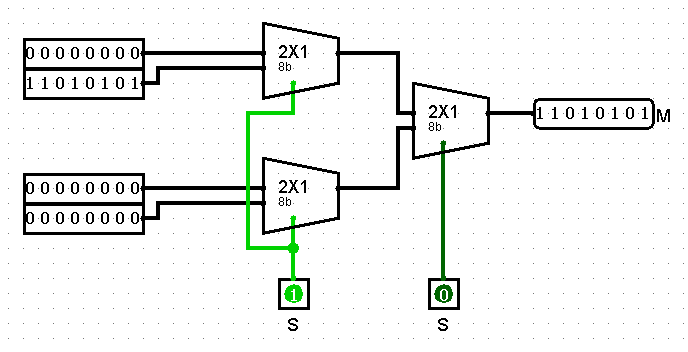
\includegraphics[scale=0.6]{mux418teste.png}
	\end{center}
\caption{\label{mux418teste}Exemplo de escolha no multiplexador 4:1 de 8 bits.}
\end{figure}

\item {MUX 8:1 8 bit}
\begin{figure}[H]
	\begin{center}
	    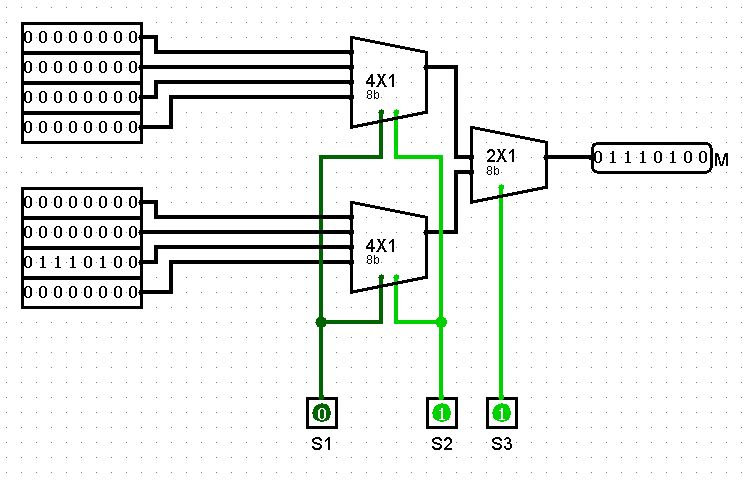
\includegraphics[scale=0.6]{mux818teste.png}
	\end{center}
\caption{\label{mux818teste}Exemplo de escolha no multiplexador 8:1 de 8 bits.}
\end{figure}

\end{itemize}

\newpage

\section{Operações na ULA de 8 bits}


\begin{itemize}
\item {OP 000 - ADD}

\begin{figure}[H]
	\begin{center}
	    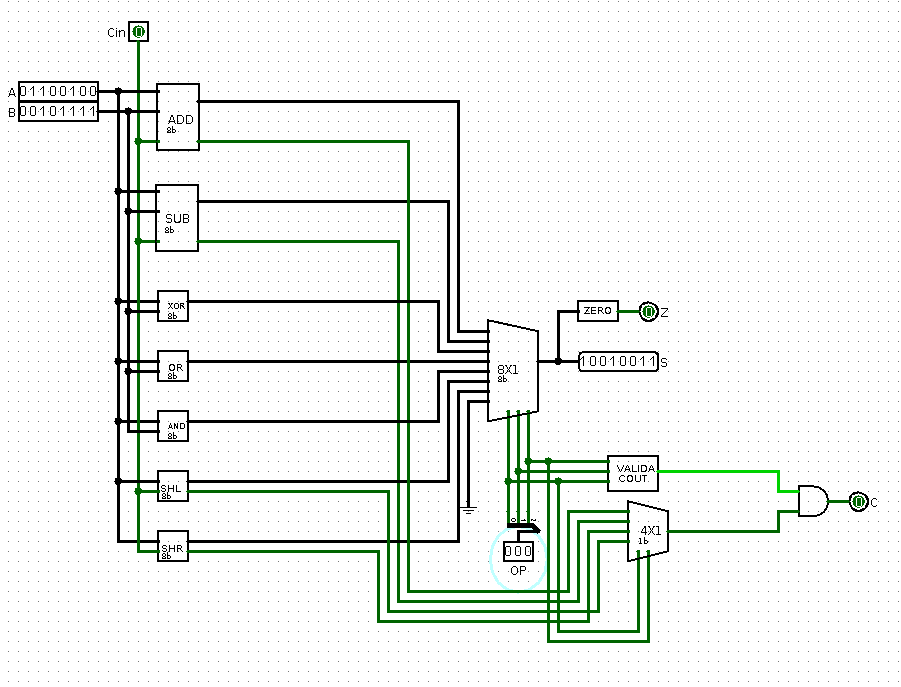
\includegraphics[scale=0.5]{alu8000add.png}
	\end{center}
\caption{\label{alu8000add}Exemplo de uma operação ADD na ULA de 8 bits.}
\end{figure}

\newpage
\item{OP 001 - SUB}

\begin{figure}[H]
	\begin{center}
	    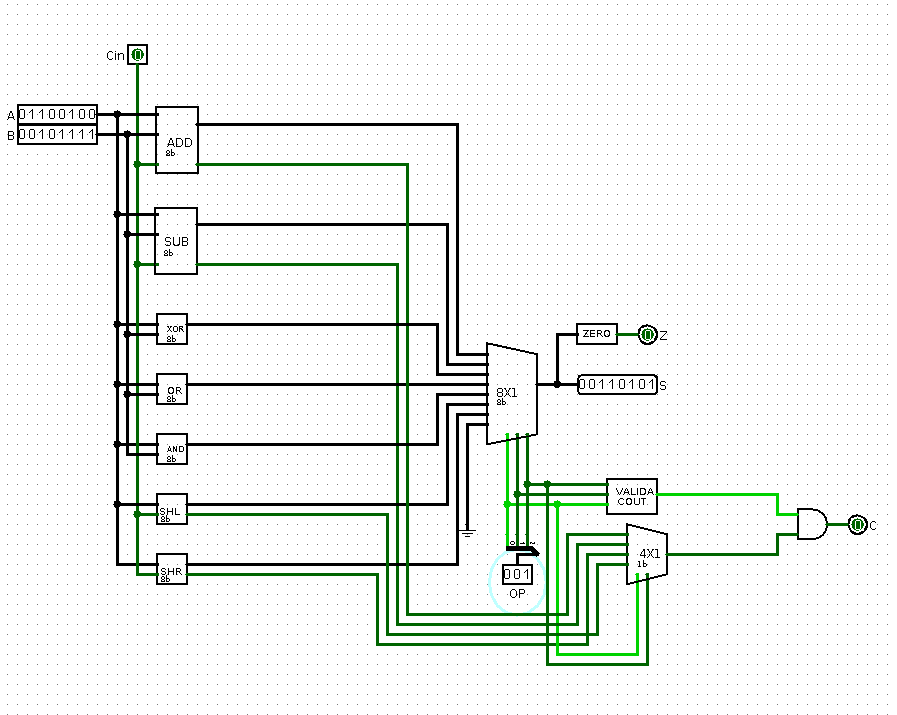
\includegraphics[scale=0.5]{alu8001sub.png}
	\end{center}
\caption{\label{alu001sub}Exemplo de uma operação SUB na ULA de 8 bits.}
\end{figure}

\newpage
\item{OP 010 - XOR}

\begin{figure}[H]
	\begin{center}
	    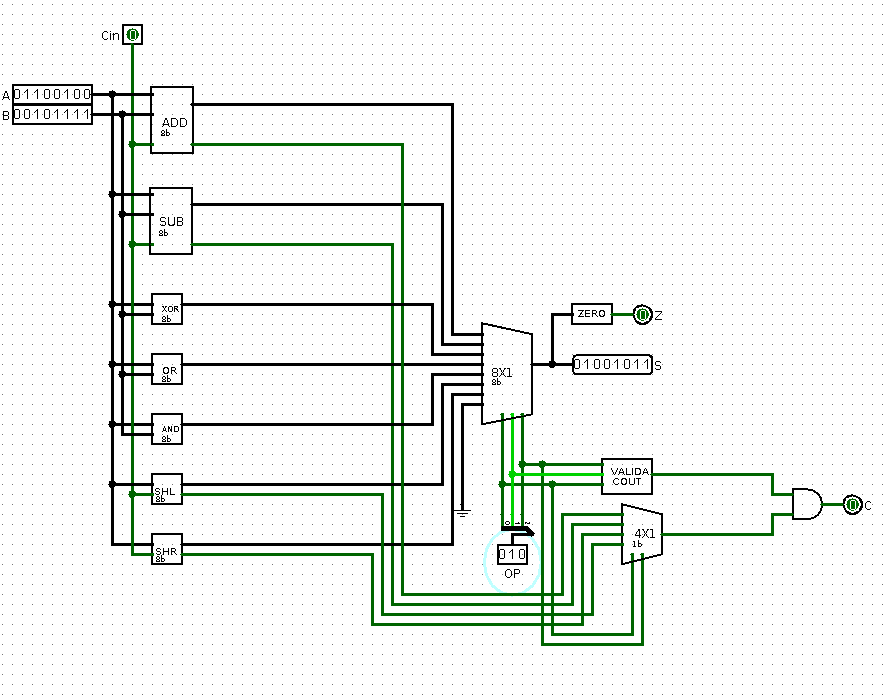
\includegraphics[scale=0.5]{alu8010xor.png}
	\end{center}
\caption{\label{alu8010xor}Exemplo de uma operação XOR na ULA de 8 bits.}
\end{figure}

\newpage
\item{OP 011 - OR}

\begin{figure}[H]
	\begin{center}
	    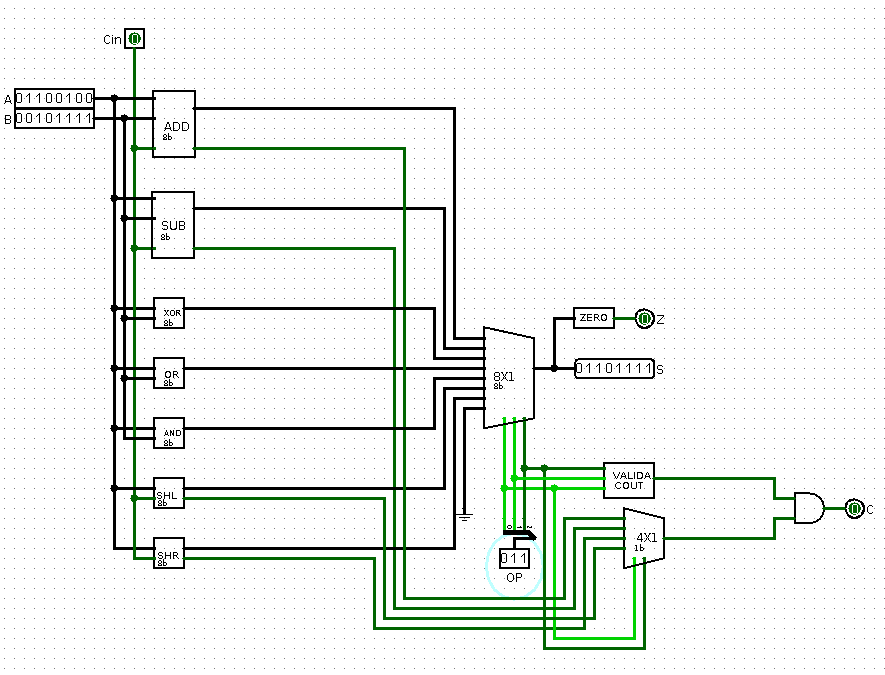
\includegraphics[scale=0.5]{alu8011or.png}
	\end{center}
\caption{\label{alu8011or}Exemplo de uma operação OR na ULA de 8 bits.}
\end{figure}

\newpage
\item{OP 100 - AND}

\begin{figure}[H]
	\begin{center}
	    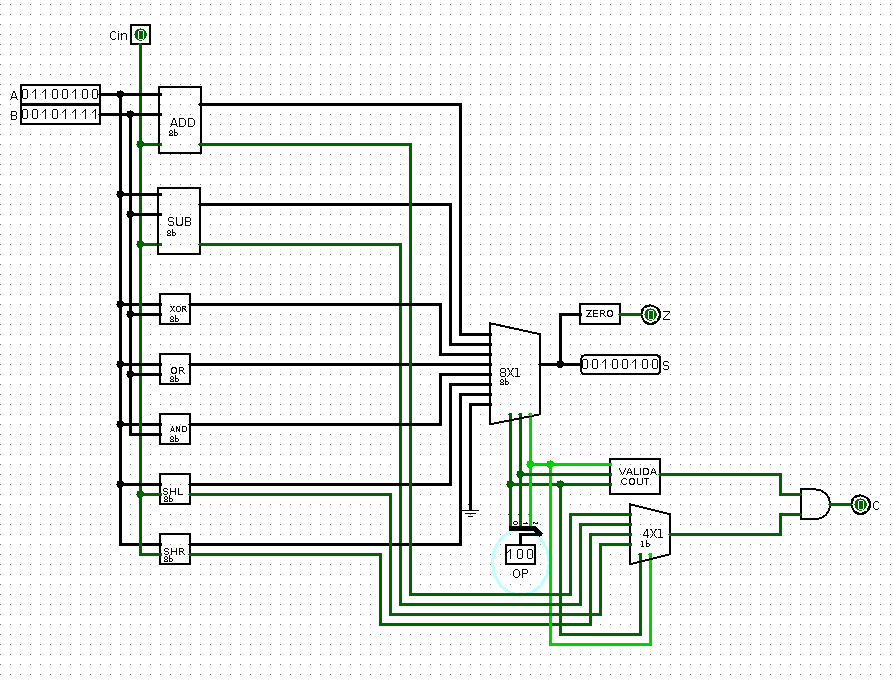
\includegraphics[scale=0.5]{alu8100and.png}
	\end{center}
\caption{\label{alu8100and}Exemplo de uma operação AND na ULA de 8 bits.}
\end{figure}

\newpage
\item{OP 101 - SHL}

\begin{figure}[H]
	\begin{center}
	    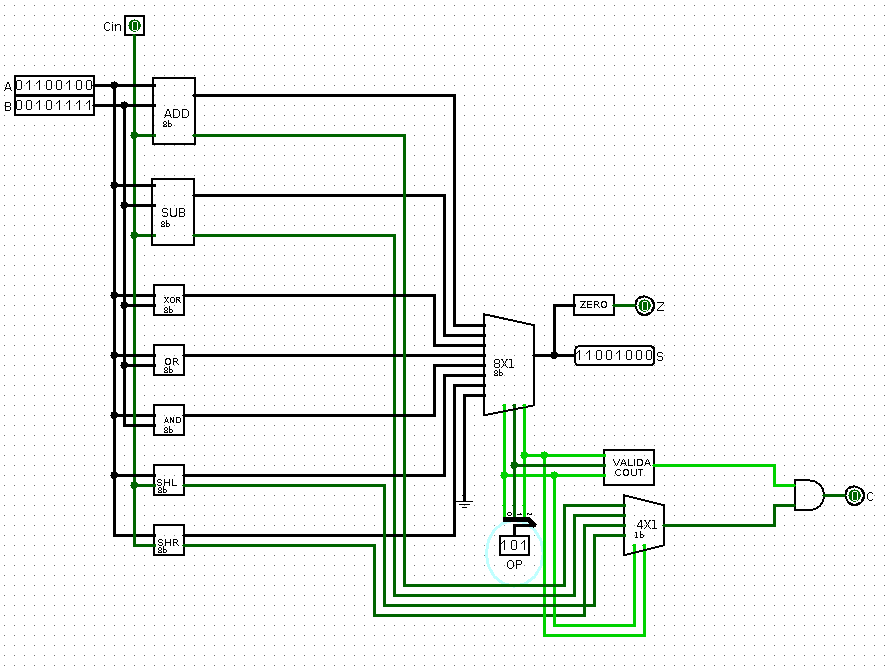
\includegraphics[scale=0.5]{alu8101shl.png}
	\end{center}
\caption{\label{alu8101shl}Exemplo de uma operação SHL na ULA de 8 bits.}
\end{figure}

\newpage
\item{OP 110 - SHR}

\begin{figure}[H]
	\begin{center}
	    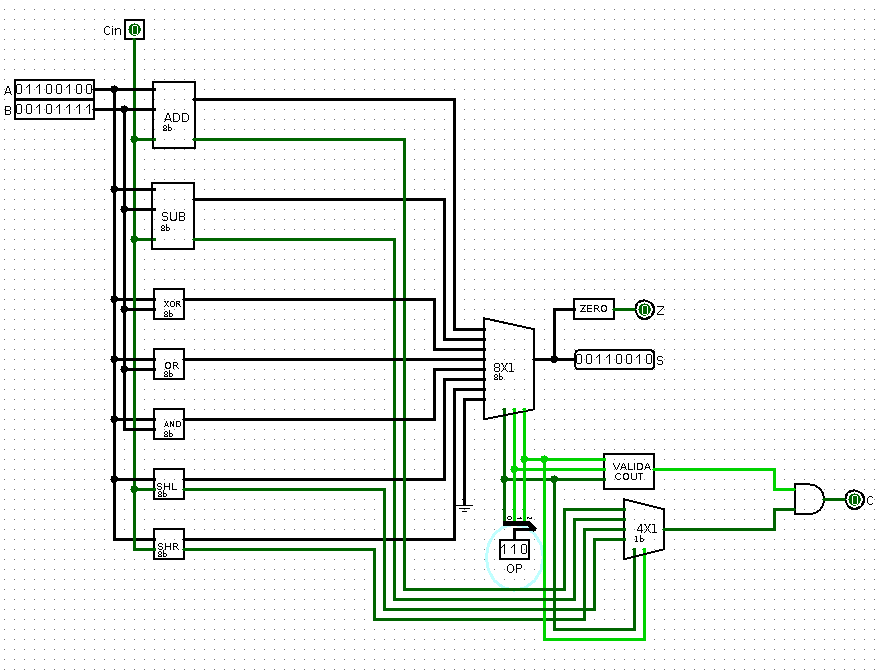
\includegraphics[scale=0.5]{alu8110shr.png}
	\end{center}
\caption{\label{alu8110shr}Exemplo de uma operação SHR na ULA de 8 bits.}
\end{figure}

\end{itemize}


\newpage
\section{Operações na calculadora}

\begin{itemize}
\item {OP 000 - ADD}

\begin{figure}[H]
	\begin{center}
	    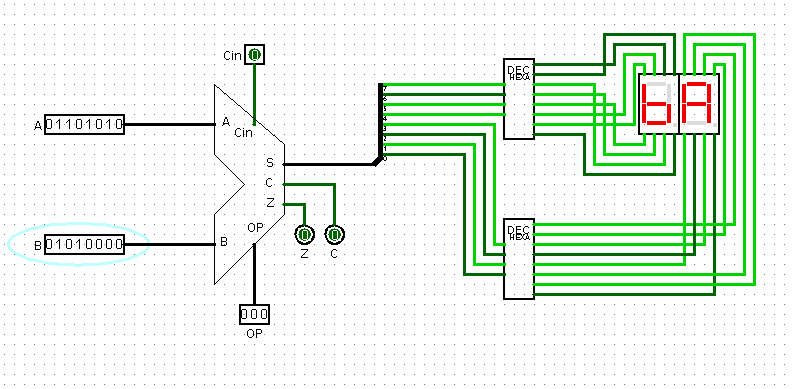
\includegraphics[scale=0.55]{calc000add.png}
	\end{center}
\caption{\label{calc000add}Exemplo de uma operação ADD na calculadora.}
\end{figure}

\item{OP 001 - SUB}

\begin{figure}[H]
	\begin{center}
	    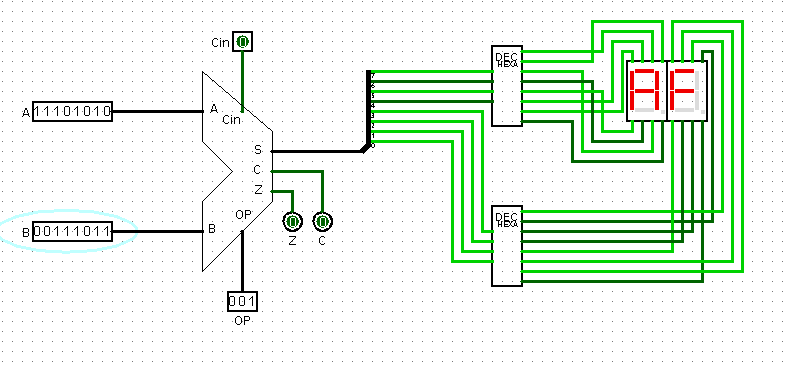
\includegraphics[scale=0.55]{calc001sub.png}
	\end{center}
\caption{\label{calc001sub}Exemplo de uma operação SUB na calculadora}
\end{figure}

\newpage
\item{OP 010 - XOR}

\begin{figure}[H]
	\begin{center}
	    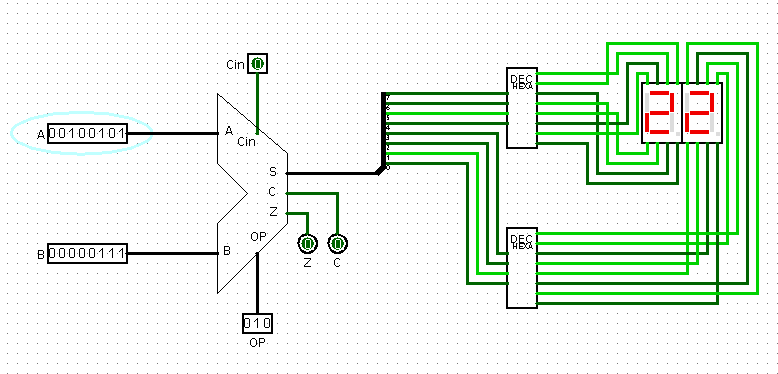
\includegraphics[scale=0.55]{calc010xor.png}
	\end{center}
\caption{\label{calc010xor}Exemplo de uma operação XOR na calculadora}
\end{figure}

\item{OP 011 - OR}

\begin{figure}[H]
	\begin{center}
	    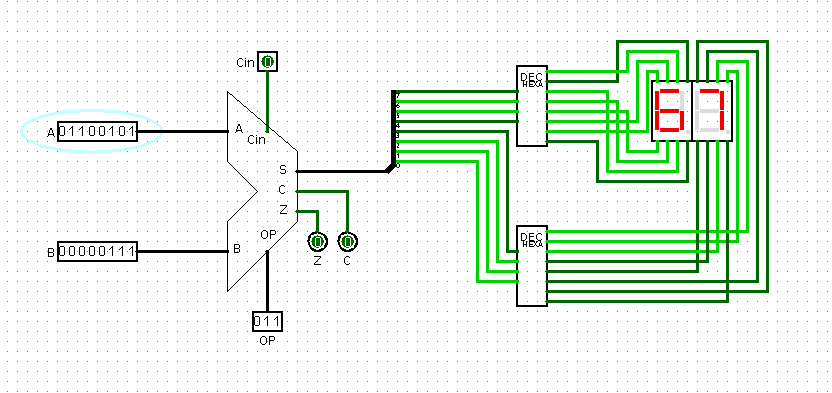
\includegraphics[scale=0.55]{calc011or.png}
	\end{center}
\caption{\label{calc011or}Exemplo de uma operação OR na calculadora}
\end{figure}

\newpage
\item{OP 100 - AND}

\begin{figure}[H]
	\begin{center}
	    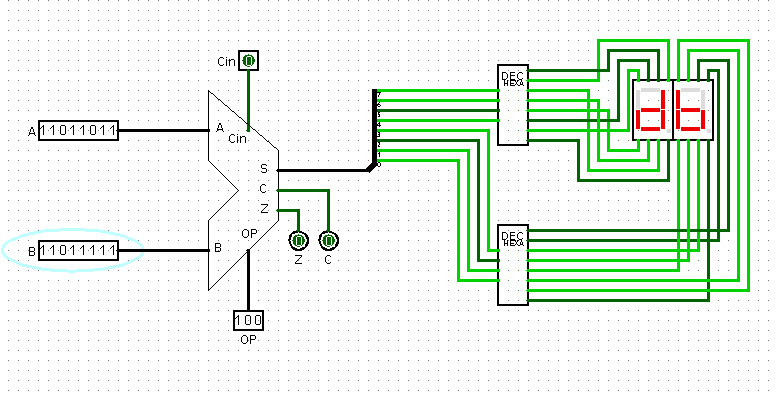
\includegraphics[scale=0.55]{calc100and.png}
	\end{center}
\caption{\label{calc100and}Exemplo de uma operação AND na calculadora}
\end{figure}

\item{OP 101 - SHL}

\begin{figure}[H]
	\begin{center}
	    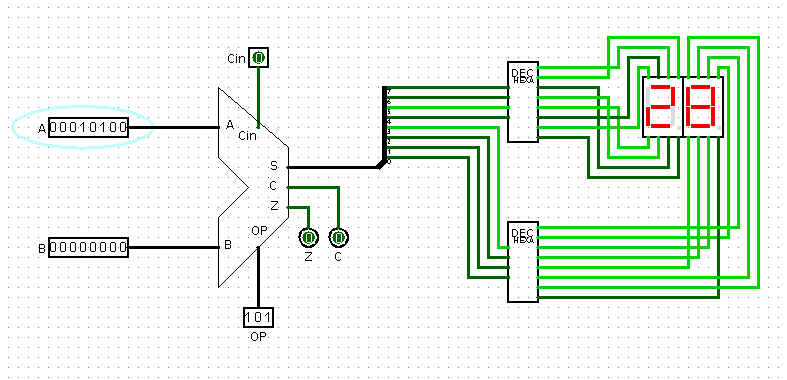
\includegraphics[scale=0.55]{calc101shl.png}
	\end{center}
\caption{\label{calc101shl}Exemplo de uma operação SHL na calculadora}
\end{figure}

\newpage
\item{OP 110 - SHR}

\begin{figure}[H]
	\begin{center}
	    \includegraphics[scale=0.55]{calc110shr.png}
	\end{center}
\caption{\label{calc110shr}Exemplo de uma operação SHR na calculadora}
\end{figure}

\end{itemize}

\newpage

\section{Operações na ULA de 16 bits}

\begin{itemize}
\item {OP 000 - ADD}

\begin{figure}[H]
	\begin{center}
	    \includegraphics[scale=0.6]{ULA16Soma.png}
	\end{center}
\caption{\label{ula16add}Exemplo de uma operação ADD na ULA DE 16 bits}
\end{figure}

\newpage
\item{OP 001 - SUB}

\begin{figure}[H]
	\begin{center}
	    \includegraphics[scale=0.6]{ULA16SUB.png}
	\end{center}
\caption{\label{ula16sub}Exemplo de uma operação SUB na ULA de 16 bits}
\end{figure}

\newpage
\item{OP 010 - XOR}

\begin{figure}[H]
	\begin{center}
	    \includegraphics[scale=0.6]{ULA16XOR.png}
	\end{center}
\caption{\label{ula16xor}Exemplo de uma operação XOR na ULA de 16 bits}
\end{figure}


\newpage
\item{OP 011 - OR}

\begin{figure}[H]
	\begin{center}
	    \includegraphics[scale=0.6]{ULA16OR.png}
	\end{center}
\caption{\label{ula16or}Exemplo de uma operação OR na ULA de 16 bits}
\end{figure}

\newpage
\item{OP 100 - AND}

\begin{figure}[H]
	\begin{center}
	    \includegraphics[scale=0.6]{ULA16AND.png}
	\end{center}
\caption{\label{ula16and}Exemplo de uma operação AND na ULA de 16 bits}
\end{figure}

\newpage
\item{OP 101 - SHL}
\begin{figure}[h]
	\begin{center}
	    \includegraphics[scale=0.6]{ULA16SHL.png}
	\end{center}
\caption{\label{ula16shl}Exemplo de uma operação SHL na ULA de 16 bits}
\end{figure}

\begin{figure}[p]
	\begin{center}
	    \includegraphics[scale=0.6]{ULA16SHL_2.png}
	\end{center}
\caption{\label{ula16shl2}Outro exemplo de uma operação SHL na ULA de 16 bits}
\end{figure}

\newpage
\item{OP 110 - SHR}
\begin{figure}[h]
	\begin{center}
	    \includegraphics[scale=0.6]{ULA16SHR.png}
	\end{center}
\caption{\label{ula16shr}Exemplo de uma operação SHR na ULA de 16 bits}
\end{figure}

\begin{figure}[p]
	\begin{center}
	    \includegraphics[scale=0.6]{ULA16SHR_2.png}
	\end{center}
\caption{\label{ula16shr2}Outro exemplo de uma operação SHR na ULA de 16 bits}
\end{figure}

\end{itemize}

\end{apendicesenv}

\end{document}
